% !TEX encoding = UTF-8 Unicode
\documentclass[11p, a4papert]{article}

\usepackage{rotating}
\usepackage[utf8]{inputenc}
\usepackage[T1]{fontenc}
\usepackage[francais]{babel}
\usepackage{multicol}
\usepackage{amsmath}
\usepackage{geometry}
\usepackage{xcolor}
\usepackage[some]{background}
\usepackage{graphics}
\usepackage{graphicx}
\usepackage{stmaryrd}
\DeclareMathOperator{\sinc}{sinc}
\usepackage{lmodern}
\usepackage{verbatim}
\usepackage{lipsum}

%Pour faire des dessins : tikz
\usepackage{pgf}
\usepackage{pgfgantt}
\usepackage{tikz}
\usetikzlibrary{arrows,automata}

\definecolor{titlepagecolor}{cmyk}{1,.60,0,.40}

\backgroundsetup{
scale=1,
angle=0,
opacity=1,
contents={\begin{tikzpicture}[remember picture,overlay]
 \path [fill=titlepagecolor] (current page.west)rectangle (current page.north east); 
 \draw [color=white, very thick] (5,0)--(5,0.5\paperheight);
\end{tikzpicture}}
}

\makeatletter                   
\def\printauthor{%                  
    {\large \@author}}          
\makeatother

\author{%
    Anthony Delannoy \\
    %Department name \\
    \texttt{anthony.delannoy@etu.enseeiht.fr}\vspace{40pt} \\
    Benoit Madiot \\
    %Department name \\
    \texttt{benoit.madiot@etu.enseeiht.fr}\vspace{40pt} \\
    Jérôme Combaniere \\
    %Department name \\
    \texttt{jerome.combaniere@etu.enseeiht.fr} 
    }

%première page
\begin{document}

\begin{titlepage}
\BgThispage
\newgeometry{left=1cm,right=6cm,bottom=3cm}
\vspace*{0.4\textheight}
\noindent
\textcolor{white}{\huge\textbf{\textsf{Méthode de lissage appliquées aux trajectoires ARGOS}}}
\vspace*{3cm}\par
\noindent
\begin{minipage}{0.5\linewidth}
    \begin{flushright}
        \printauthor
    \end{flushright}
\end{minipage} \hspace{15pt}
%
\begin{minipage}{0.02\linewidth}
    \rule{1pt}{175pt}
\end{minipage} \hspace{-10pt}
%
\begin{minipage}{0.63\linewidth}
\vspace{5pt}
    \begin{abstract} 
        Pour protéger certaines espèces maritimes menacées, le CLS équipe ces animaux de balises ARGOS. Le présent rapport vise à expliquer quelles sont les méthodes qui ont été mises en place pour pouvoir obtenir des trajectoires lisses représentatives des lieux de vie de ces animaux.
    \end{abstract}
\end{minipage}
\end{titlepage}
\restoregeometry

%Table des matieres
\newpage
\thispagestyle{empty}
\tableofcontents
\newpage

%%%%%%%Debut du contenu%%%%%%%

\part{Introduction}
\paragraph{}
 Ce rapport est écrit dans le cadre du projet long de troisième année à l'ENSEEIHT. Pendant six semaines nous avons travaillé en collaboration avec le CLS pour convertir leur programme de lissage de position ARGOS du langage Matlab vers le langage Python.
\paragraph{}
La partie code de notre projet se répartit en deux grandes parties : la première de lecture/ecriture dans les différents types de fichiers que fournit le programme ARGOS et la deuxième de fonctions lissages à proprement parler.
\paragraph{}
Nous tenons à remercier Beatriz Calmettes, notre superviseur au sein du CLS pour sa disponibilité et son aide précieuse tout au long du stage ainsi que Philippe Gaspar pour ses pistes de recherches et ses livres qui nous ont aidé pour faire aboutir notre travail.
\newpage
\part{Code}
\section{RWFormats}
\subsection{Lecture des fichiers}
\subsubsection{Mise en format commun}

\paragraph{}
Nous avons trois formats de fichiers à disposition : diag, ds et csv. Afin de simplifier l'écriture des algorithmes de lissages nous avons une fonction s'occupant d'identifier le format du fichier, d'y appliquer la bonne méthode de lecture puis retourner notre \emph{format commun}.

\paragraph{Format d'une transmission}
Les éléments essentiels d'une transmission sont stockés dans un dictionnaire respectant l'architecture ci-dessous. Les éléments sont tous des strings sauf "date" qui est un dictionnaire.
\vspace{1cm}
\begin{center}
$uneTransmission = \left\{\begin{array}{c} "date" \\"LC" \\"lat" \\"lon" \\"lat\_image" \\"lon\_image" \\ \end{array}\right\}$
\end{center}

\paragraph{Format du dictionnaire des dates}
\begin{center}
$dicoDate = \left\{\begin{array}{c} "annee" \\"mois" \\"jour" \\"heure" \\"min" \\"sec" \\ \end{array}\right\}$
\end{center}

\paragraph{}
L'utilisation des dictionnaires permettent un rangement et une récupération des données simplifiés, il suffit de connaître la clé de la donnée pour y accéder.

\paragraph{Format des transmissions de tout un fichier}
Comme nous l'avons vu, chaque transmission est stockée comme un dictionnaire. Afin de les ranger dans l'ordre nous les mettons ensuite dans une liste. 

\begin{center}
$formatCommun = \left[\begin{array}{cccc} dico[1] & dico[2] & ... & dico[n] \\ \end{array}\right]$
\end{center}

%\subsubsection{Format DIAG}
%\subsubsection{Format DS}
%\subsubsection{Format CSV}
\subsubsection{Format XML}
\paragraph{}
Nous avons créé une fonction readXml permettant de lire les fichiers XML regroupant les caractéristiques principales de chaque espèce. Ces paramètres sont alors mis dans un dictionnaire pour un accès simple.

%\subsection{Écriture des fichiers} % à laisser ?
\section{Utilities}
\subsection{Suppression des outliers}
\paragraph{}
Le système ARGOS faisant parfois des erreurs dans le choix de la bonne localisation (entre le couple latitude, longitude et latitude image, longitude image) nous appliquons un algorithme simple aux données. Nous choisissons toujours la plus petite distance entre deux points, cela permet d'éliminer les données abhérantes.

\subsection{Suppression des vitesses excessives}
\paragraph{}
Afin d'enlever les données eronnées qui peuvent rester dans les localisations, il est nécessaire de mettre en place un algorithme permettant d'éliminer les points responsables d'une vitesse aberrante. C'est le rôle de la fonction que l'on a codée en Python suppVitesseExcess. La fonction permet de calculer la vitesse entre deux points de la trajectoire et compare cette dernière avec la vitesse maximale de l'espèce étudiée en prenant également en compte la classe de localisation des points. Si la vitesse calculée est supérieure à la vitesse seuil, le point est alors supprimé. 
Elle prend en argument d'entrée:

\begin{itemize}
\item la liste des points
\item la fonction recuperation permettant d'accéder aux informations des dicos
\item la fonction convertArrayOfTime qui convertit en secondes une date
\item la fonction calculVitesses qui permet de calculer une vitesse étant donnée une liste de latitudes,longitudes,d'instants
\item une vitesse maximale seuil
\end{itemize}
\newpage




\begin{tabular}{cc}
   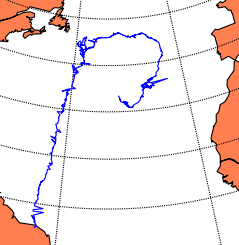
\includegraphics[scale=0.85]{avecCorrecDistance.png}
   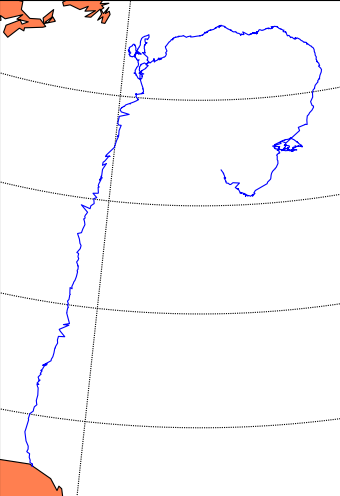
\includegraphics[scale=0.45]{avecVitEx.png}
\end{tabular}
\begin{figure}
 \begin{minipage}[b]{.46\linewidth}

  \caption{Trajectoire avant suppression des vitesses excessives \label{fig1}}
 \end{minipage} \hfill
 \begin{minipage}[b]{.46\linewidth}
  
  \caption{Trajectoire après suppression des vitesses excessives \label{fig2}}
 \end{minipage}
\end{figure}
\newline
\newline
\newline
\subsection{Estimation 1}
\paragraph{}
Cette première estimation estime chaque point de la trajectoire (excepté les deux premiers et les deux derniers) comme une somme pondérée du point à estimer et des deux points précédents et des deux points suivants. Cette pondération dépend à la fois de la précision de la localisation et d'un noyau. Nous n'utilisons que cinq points pour l'estimation puisqu'une étude antérieure a montré que les résultats obtenus pour ce nombre de points sont sensiblement les mêmes que pour un nombre de points plus importants.
\newline
En ce qui concerne le noyau, nous avons préférentiellement utilisé le noyau d'Epanechnikov puisqu'il minimise l'AMISE (Asymptotic Integrated Mean Squarred Error), ce qui représente l'efficacité d'un noyau, mais nous également codé un noyau gaussien pour pouvoir comparer les résultats.
\newline
%\newpage
Le poids associé à la précision de la localisation est linéaire : plus la localisation est précise plus le poids associé est important. C'est un simple ajout d'information pour que le programme se fie plus aux localisations précises qu'aux localisations imprécises.
\newline
Si le point estimé après calcul est trop éloigné de la position de base, on retire simplement cette position. Cette regression permet de lisser les pics qui ressortent le long de la trajectoire. 

\subsection{Estimation 2}
\paragraph{}
En plus de la première estimation, nous avons également réalisé une seconde estimation, estimation2. Celle-ci, comme la première, effectue une régression linéaire à l'aide d'une fenêtre dont les paramètres sont contenus dans les fichiers XML et sont spécifiques à chaque espèce. Les trous où l'estimation n'a pas été possible sont comblés en approximant par une droite grâce à la fonction comblerTrous. Cette fonction permet aussi de réaliser un rééchantillonage de la courbe selon un pas d'échantillonnage constant, i.e. les points de la trajectoire sont au final espacés d'un intervalle de temps constant.
Cette fonction prend comme arguments d'entrée:
\begin{itemize}
\item la liste des points
\item la taille de la demi-fenêtre
\item la taille maximale de la demi-fenêtre
\item le nombre de points dans la demi-fenêtre
\item le pas d'échantillonnage
\item le nombre minimum de points dans la fenêtre pour pouvoir effectuer une estimation
\item la fonction recuperation permettant d'accéder aux informations contenues dans le dico
\item la fonction convertArrayOfTime qui convertit en secondes une date
\item la fonction kernel permettant de calculer les poids, nécessaires pour la régression linéaire, grâce aux kernels
\item la fonction comblerTrous permettant de combler les trous de l'estimation en approximant par une droite
\item la fonction convertSecondToDatetime permettant de convertir un instant (en secondes) en une date
%\newpage
\end{itemize}
\vspace{0.5cm}
\begin{tabular}{cc}
   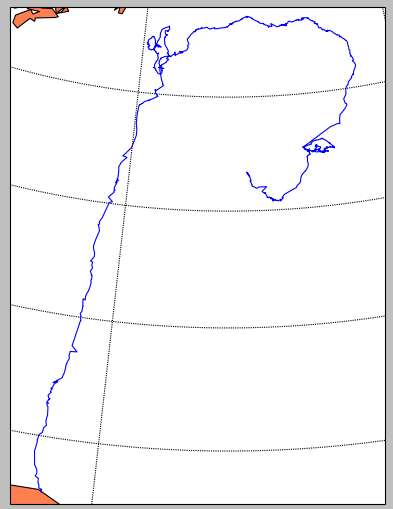
\includegraphics[scale=0.45]{SansEst2.png}
   \hspace{2cm}
   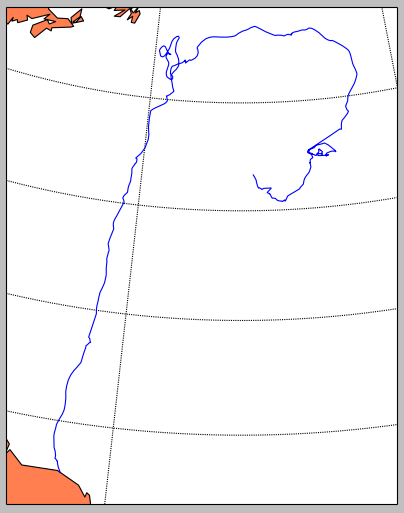
\includegraphics[scale=0.45]{AvecEst2.png}
\end{tabular}
\begin{figure}[h!]
 \begin{minipage}[b]{.46\linewidth}

  \caption{Trajectoire avant estimation2 \label{fig1}}
 \end{minipage} \hfill
 \begin{minipage}[b]{.46\linewidth}
  
  \caption{Trajectoire après estimation2 \label{fig2}}
 \end{minipage}
\end{figure}

\newpage
\subsection{Lissage de Kalman}
\paragraph{}
Le lissage de Kalman se base sur une connaissance à priori des états de nore système et sur une observation de ces états. Dans notre cas, l'état correspond à trois grandeurs : la latitude, la longitude et la vitesse. 

\paragraph{}
La matrice de transition permettant de passer d'un état à l'état suivant est estimée en utilisant un algorithme EM (Expectation Maximization) suite à un manque de temps pour la coder nous mêmes. 
\paragraph{}
A la différence d'un filtre de Kalman (comme le schéma ci-dessous) qui ne se base que sur les données actuelles et qui se met donc à jour à chaque nouvelle arrivée de données, le lisseur de Kalman utilise dès le début l'ensemble de toutes les données ainsi que la connaissance à priori pour fournir une courbe lisse qui correspond au mieux à nos observations ainsi qu'à la dynamique du système.
\newline
\newline
\newline

\begin{figure}[h!]
\centering
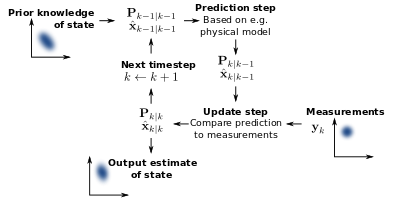
\includegraphics[scale=0.8]{klman.png}
\caption{Schéma de fonctionnement d'un filtre de Kalman}
\end{figure}

\newpage
\part{Interface graphique}

\begin{figure}[h!]
\centering
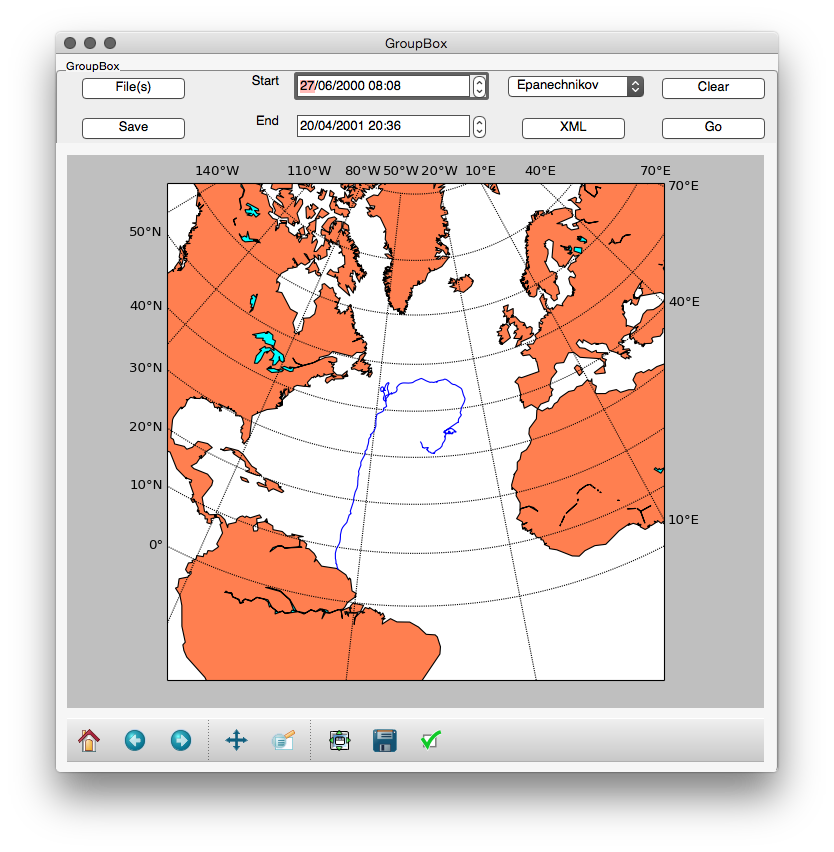
\includegraphics[scale=0.5]{gui.png}
\caption{Interface graphique.}
\end{figure}


\paragraph{}
L'interface permet de simplifier l'usage de toutes les méthodes discutées plus haut. Ainsi elle permet de tracer une ou plusieurs courbes sur une carte simplifiée : grâce au bouton "File(s)" on choisit le ou les fichiers puis le bouton "Go" lance les calculs. Si l'on veut les effacer et retrouver une carte "propre" il suffit d'appuyer sur le bouton "Clear" puis de retracer des courbes. 

\paragraph{}
Le bouton XML permet de choisir son fichier de paramètre donnant par exemple la vitesse maximum de l'espèce, le pas d'échantillonnage, les tailles de fenêtre pour les estimations...

\paragraph{}
Le choix du filtre se fait par un menu déroulant, nous avons implémenté trois filtres : Epanechnikov, Gaussien et Kalman.

\paragraph{}
Il y a possibilité de filtrer les données par dates. Les données sont alors tronquées et seul ce qui est dans les limites est pris en compte.

\paragraph{}
Finalement les données post-traitement peuvent être sauvegarder grâce au bouton "Save". Des fichiers res sont alors créés dans le dossier Python/res/ \\
Les noms de ces fichiers sont l'identifiant de la balise suivi du nom du filtre utilisé (par exemple "10248-epan.res").

\newpage
\part{Conclusion}

\paragraph{}
Nos programmes sont robustes et fiables et le travail fourni jusqu'à présent tend à encadrer les espèces menacées en générant de façon fiable leurs trajectoires.
\newline
L'interface graphique permet également d'afficher et de travailler sur plusieurs courbes à la fois.
\paragraph{}
Notre travail ouvre par ailleurs les portes vers de nouvelles pistes de recherches comme :
\begin{itemize}
\item la comparaison entre les différentes méthodes de lissage
\item la prise en charge des derniers formats de fichiers ARGOS
\item l'évolution du programme avec Python 3
\end{itemize}








\end{document}